\section{Application Layer}

\subsubsection{Netzwerk-Applikationen und Protokolle}

\begin{KR}{Übersicht Applikationsprotokolle}
    \begin{itemize}
        \item Das Domain Name System (DNS) erlaubt übersetzt Hostnamen in IP Adressen und umgekehrt
        \begin{itemize}
            \item Besteht aus einem hierarchischen DNS Name Space
            \item Das DNS wird auf einer grossen Anzahl Name Server verteilt betrieben, ein Name Server ist jeweils für eine Zone verantwortlich (z.B. zhaw.ch)
        \end{itemize}
        \item DHCP erlaubt einem Rechner, seine IP Konfiguration von einem Server zu beziehen
        \item TFTP ist ein einfaches, aber zuverlässiges File Transfer Protocol, welches z.B. diskless Systemen dazu dient, das Betriebssystem Image vom Server zu beziehen
        \item HTTP erlaubt den Zugriff auf verteilte Dokumente, die mittels Uniform Resource Locator (URL) eindeutig adressiert werden
        \item Network Address Translation (NAT) erlaubt die Wiederverwendung privater IP-Adressen
    \end{itemize}
\end{KR}

\subsubsection{DNS - Domain Name System}

\begin{definition}{DNS - Domain Name Space}
    \begin{itemize}
        \item Leserliche Darstellung von IP-Adressen (Name Resolution)
        \item Hauptdomäne = Root
        \item Der Fully Qualified Domain Name (FQDN) muss eindeutig sein, Beispiel: sw.eng.
        \item Geschwisterknoten dürfen nicht den gleichen Namen haben
    \end{itemize}
    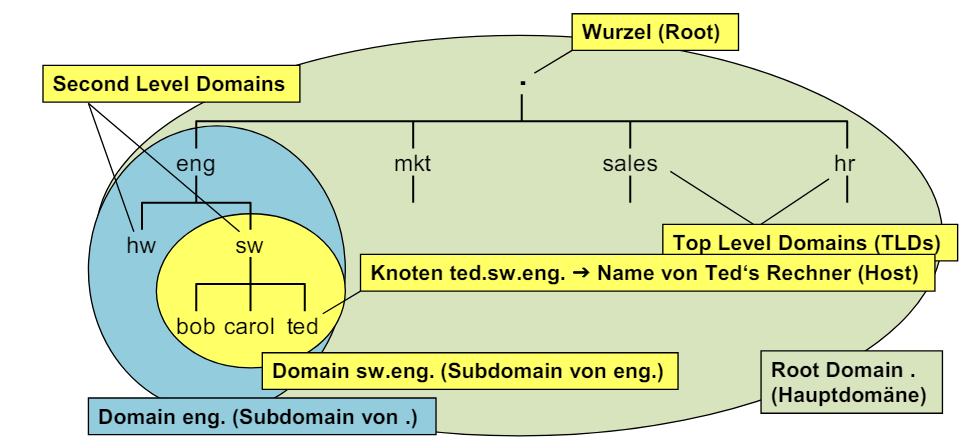
\includegraphics[width=1\linewidth]{images/dns_explained.png}
\end{definition}

\begin{concept}{Verwaltung von Domains}
    \begin{itemize}
        \item Das DNS wird verteilt betrieben (verteilt, nicht repliziert)
        \item Ein Name Server ist meist für eine Zone verantwortlich
        \begin{itemize}
            \item Zone: separat administrierter Subtree des DNS
            \item Ein Name Server kennt
            \begin{itemize}
                \item die IP-Adressen zu den Hostnamen in seiner Zone
                \item die IP-Adressen der Name Server seiner Subdomänen, falls diese nicht in seiner Zone liegen
                \item die IP-Adressen von Root und TLD Name Server, um beliebige Abfragen zu erlauben
            \end{itemize}
        \end{itemize}
        \item Aus Redundanzgründen min. zwei Name Server für eine Zone
        \begin{itemize}
            \item Primary (Master) und Secondary (Slave) 
        \end{itemize}
        \item Ein NS kann eine Unterzone seiner Zone weiter delegieren
    \end{itemize}
\end{concept}

\begin{definition}{DNS Record Types}\\
    Der "Record Type" enthält Information, welche Daten angefragt beziehungsweise in einer
    Antwort vom Name Server mitgeteilt werden\\
    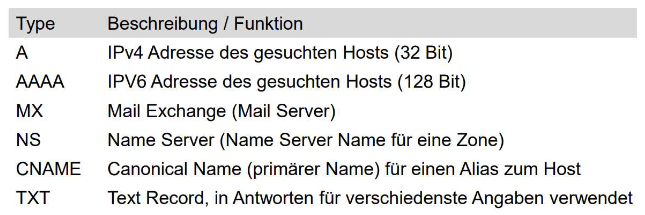
\includegraphics[width=1\linewidth]{images/dns_record_types.png}
\end{definition}

\begin{definition}{Reverse DNS Lookup}\\
    Authentisierung: Ein Server identifiziert/authentifiziert einen Client anhand des Namens, nicht anhand der IP-Adresse
\end{definition}

\begin{example2}{DNS-Abfragen auswerten}
    \begin{itemize}
        \item DNS verwendet Port 53 (UDP)
        \item Resolver: lokale Software, die mit dem Name Server kommuniziert
    \end{itemize}
    Beispiel: Anwendung benötigt die IP-Adresse von bob.sw.eng.
    \begin{itemize}
        \item FQDN: bob.sw.eng. 
        \item Root: .
        \item Top Level Domain: eng
        \item Second Level Domain: sw
    \end{itemize}
        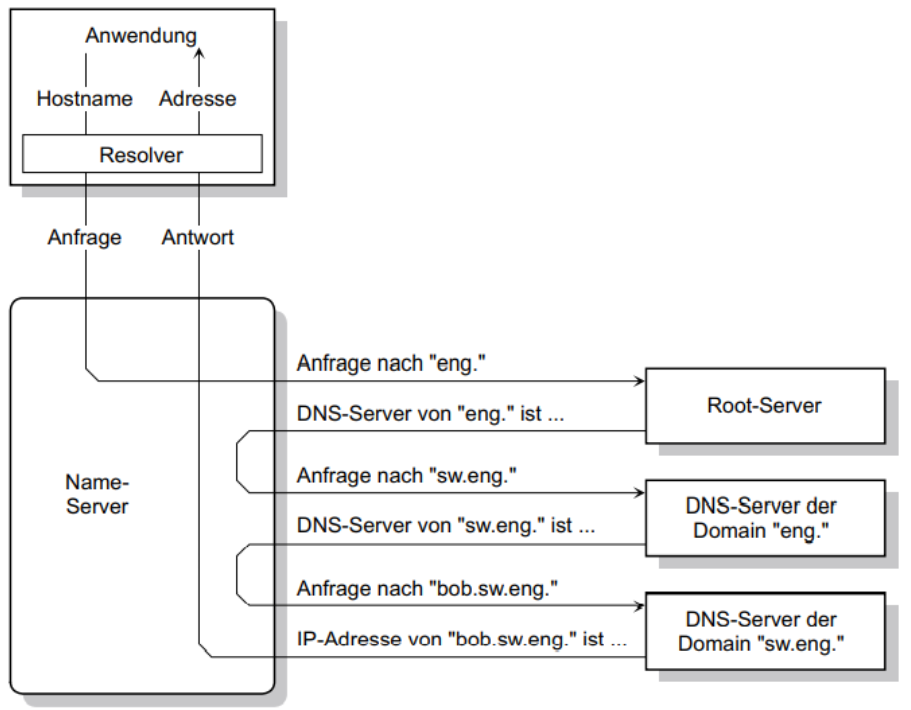
\includegraphics[width=1\linewidth]{images/example_dns.png}        
\end{example2}

\columnbreak

\subsubsection{NAT - Network Address Translation}

\begin{definition}{NAT (Port Mapping)}\\
    Alle Hosts im privaten Netz 192.168.0.0/8 verwenden 192.168.0.1 als Default-Gateway.\\
    Port-basierte NAT (NAPT) hat folgende Funktionen:
    \begin{itemize}
        \item Ersetzt private IP Adresse im IP Header durch eine öffentliche IP des Gateways / Routers
        \item Ersetzt die private Port-Nr. des Hosts durch eine freie zulässigen Port-Nr. des Gateways / Routers
        \item Erstellt ein Mapping von privater IP Adresse und Port-Nr. zur öffentlichen Port-Nr.
        \item Man kann für das Mapping auch statische Werte definieren, hier wird aber nur die Port-Nummer übernommen
    \end{itemize}
    Problem mit NAT:\\
    NAT verletzt das Konzept der OSI-Layer. Um einen Port im TCP Header zu ändern muss man eigentlich die
    Daten im IP-Frame ändern. Bedeutet eine Netzwerk-Funktion greift auf den Transport Header zu.
    IP-Adresse und Portnummer werden dabei verändert. \\
        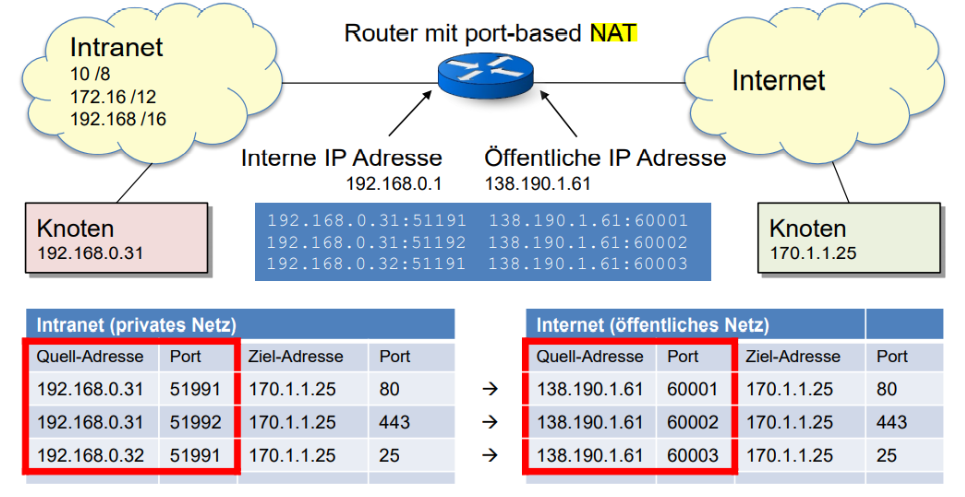
\includegraphics[width=1\linewidth]{images/NAT.png}
\end{definition}

\columnbreak

\subsection{DHCP - Dynamic Host Configuration Protocol}

\begin{definition}{Bezug IP-Adresse}\\
    Wie erhält ein Knoten seine IP-Adresse?
    \begin{itemize}
        \item Lokal konfiguriert (static IP)
        \item Bezug der IP-Adresse über das Netzwerk
        \begin{itemize}
            \item DHCP – erlaubt dynamische Zuteilung aus dem lokalen Adressbereich
        \end{itemize}
    \end{itemize}
\end{definition}

\begin{concept}{Dynamische Zuweisung von IP-Adressen}
    \begin{itemize}
        \item Client verlangt eine IP-Adresse (DHCP Request)
        \item DHCP-Server erteilt eine freie Adresse für definierte Lease Time, oft 10 Minuten (DHCP-Response)
        \item Vor Ablauf der Lease Time muss der Lease (vom Client) erneuert werden
        \item Client, der das Netz verlässt, wird Lease nicht erneuern $\rightarrow$ Adresse wieder frei
    \end{itemize}
\end{concept}



\begin{KR}{Ablauf DHCP}
    \begin{enumerate}
        \item Client sucht DHCP Server mittels Broadcast
        \item DHCP Server antwortet (DHCP offer)
        \item Der Client wählt einen Server und fordert eine Auswahl der angebotenen Parameter (DHCP request)
        \item Der Server bestätigt mit einer Message, welche die endgültigen Parameter enthält
        \item Vor Ablauf der Lease-Time erneuert der Client die Adresse.
    \end{enumerate}
\end{KR}

\columnbreak

\begin{definition}{DHCP - Dynamic Host Configuration Protocol}
    \begin{itemize}
        \item Dynamische Zuweisung von IP-Adressen
        \item Reserviert nur IP’s von aktiven Geräte
    \end{itemize}
    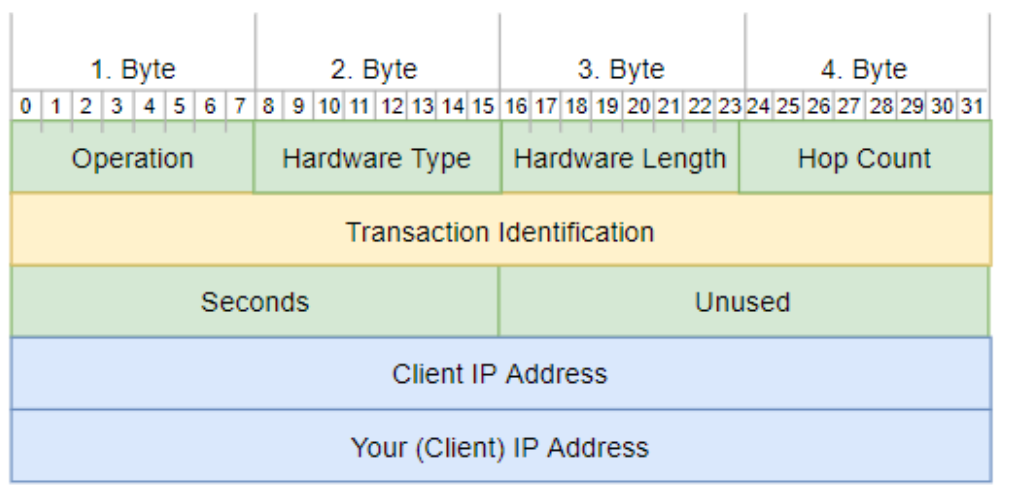
\includegraphics[width=1\linewidth]{images/bootp.png}
\end{definition}

\begin{definition}{DHCP Paketformat}\\
    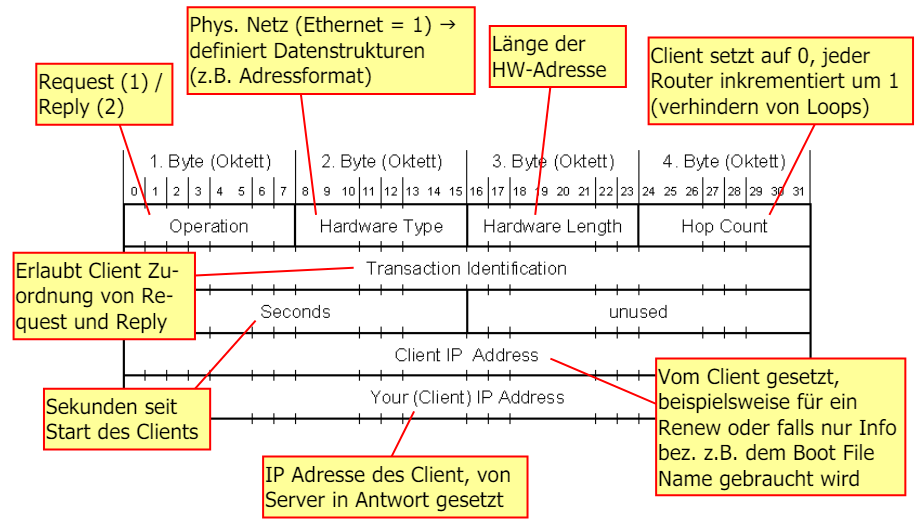
\includegraphics[width=1\linewidth]{images/dhcp_format1.png}\\
    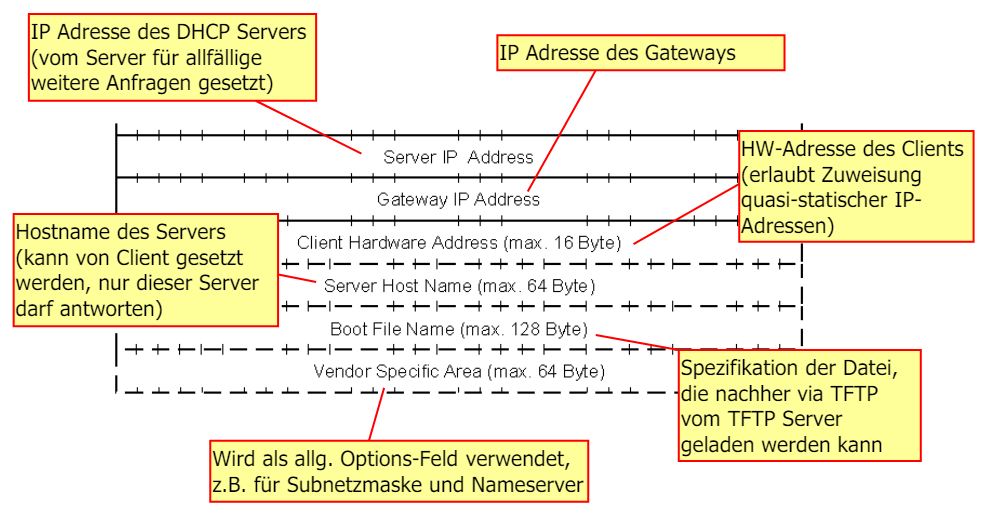
\includegraphics[width=1\linewidth]{images/dhcp_format2.png}
\end{definition}






